\documentclass{beamer}

\pdfmapfile{+sansmathaccent.map}


\mode<presentation>
{
	\usetheme{Warsaw} % or try Darmstadt, Madrid, Warsaw, Rochester, CambridgeUS, ...
	\usecolortheme{seahorse} % or try seahorse, beaver, crane, wolverine, ...
	\usefonttheme{serif}  % or try serif, structurebold, ...
	\setbeamertemplate{navigation symbols}{}
	\setbeamertemplate{caption}[numbered]
} 


%%%%%%%%%%%%%%%%%%%%%%%%%%%%
% itemize settings


%%%%%%%%%%%%%%%%%%%%%%%%%%%%
% itemize settings

\definecolor{myhotpink}{RGB}{255, 80, 200}
\definecolor{mywarmpink}{RGB}{255, 60, 160}
\definecolor{mylightpink}{RGB}{255, 80, 200}
\definecolor{mypink}{RGB}{255, 30, 80}
\definecolor{mydarkpink}{RGB}{155, 25, 60}

\definecolor{mypaleblue}{RGB}{240, 240, 255}
\definecolor{mylightblue}{RGB}{120, 150, 255}
\definecolor{myblue}{RGB}{90, 90, 255}
\definecolor{mygblue}{RGB}{70, 110, 240}
\definecolor{mydarkblue}{RGB}{0, 0, 180}
\definecolor{myblackblue}{RGB}{40, 40, 120}

\definecolor{myblackturquoise}{RGB}{5, 53, 60}
\definecolor{mydarkdarkturquoise}{RGB}{8, 93, 110}
\definecolor{mydarkturquoise}{RGB}{28, 143, 150}
\definecolor{mypaleturquoise}{RGB}{230, 255, 255}
\definecolor{myturquoise}{RGB}{48, 213, 200}

\definecolor{mygreen}{RGB}{0, 200, 0}
\definecolor{mydarkgreen}{RGB}{0, 120, 0}
\definecolor{mygreen2}{RGB}{245, 255, 230}

\definecolor{mygrey}{RGB}{120, 120, 120}
\definecolor{mypalegrey}{RGB}{160, 160, 160}
\definecolor{mydarkgrey}{RGB}{80, 80, 160}

\definecolor{mydarkred}{RGB}{160, 30, 30}
\definecolor{mylightred}{RGB}{255, 150, 150}
\definecolor{myred}{RGB}{200, 110, 110}
\definecolor{myblackred}{RGB}{120, 40, 40}


\definecolor{myblackmaroon}{RGB}{50, 0, 15}

\definecolor{mygreen}{RGB}{0, 200, 0}
\definecolor{mygreen2}{RGB}{205, 255, 200}

\definecolor{mydarkcolor}{RGB}{60, 25, 155}
\definecolor{mylightcolor}{RGB}{130, 180, 250}

\setbeamertemplate{itemize items}[default]

\setbeamertemplate{itemize item}{\color{myblackmaroon}$\blacksquare$}
\setbeamertemplate{itemize subitem}{\color{mydarkdarkturquoise}$\blacktriangleright$}
\setbeamertemplate{itemize subsubitem}{\color{mygray}$\blacksquare$}

\setbeamercolor{palette quaternary}{fg=white,bg=myblackmaroon}
\setbeamercolor{titlelike}{parent=palette quaternary}

\setbeamercolor{palette quaternary2}{fg=black,bg=mypaleblue}
\setbeamercolor{frametitle}{parent=palette quaternary2}

\setbeamerfont{frametitle}{size=\Large,series=\scshape}
\setbeamerfont{framesubtitle}{size=\normalsize,series=\upshape}





%%%%%%%%%%%%%%%%%%%%%%%%%%%%
% block settings

\setbeamercolor{block title}{bg=red!30,fg=black}

\setbeamercolor*{block title example}{bg=mygreen!40!white,fg=black}

\setbeamercolor*{block body example}{fg= black, bg= mygreen2}


%%%%%%%%%%%%%%%%%%%%%%%%%%%%
% URL settings
\hypersetup{
	colorlinks=true,
	linkcolor=blue,
	filecolor=blue,      
	urlcolor=blue,
}

%%%%%%%%%%%%%%%%%%%%%%%%%%

\renewcommand{\familydefault}{\rmdefault}

\usepackage{amsmath}
\usepackage{mathtools}

\usepackage{subcaption}

\usepackage{qrcode}

\DeclareMathOperator*{\argmin}{arg\,min}
\newcommand{\bo}[1] {\mathbf{#1}}

\newcommand{\R}{\mathbb{R}} 
\newcommand{\T}{^\top}     



\newcommand{\mydate}{Fall 2023}

\newcommand{\mygit}{\textcolor{blue}{\href{https://github.com/SergeiSa/Mechatronics-2023}{github.com/SergeiSa/Mechatronics-2023}}}

\newcommand{\myqr}{ \textcolor{black}{\qrcode[height=1.5in]{https://github.com/SergeiSa/Mechatronics-2023}}
}

\newcommand{\myqrframe}{
	\begin{frame}
		\centerline{Lecture slides are available via Github, links are on Moodle}
		\bigskip
		\centerline{You can help improve these slides at:}
		\centerline{\mygit}
		\bigskip
		\myqr
	\end{frame}
}


\newcommand{\bref}[2] {\textcolor{blue}{\href{#1}{#2}}}

%%%%%%%%%%%%%%%%%%%%%%%%%%%%
% code settings

\usepackage{listings}
\usepackage{color}
% \definecolor{mygreen}{rgb}{0,0.6,0}
% \definecolor{mygray}{rgb}{0.5,0.5,0.5}
\definecolor{mymauve}{rgb}{0.58,0,0.82}
\lstset{ 
	backgroundcolor=\color{white},   % choose the background color; you must add \usepackage{color} or \usepackage{xcolor}; should come as last argument
	basicstyle=\footnotesize,        % the size of the fonts that are used for the code
	breakatwhitespace=false,         % sets if automatic breaks should only happen at whitespace
	breaklines=true,                 % sets automatic line breaking
	captionpos=b,                    % sets the caption-position to bottom
	commentstyle=\color{mygreen},    % comment style
	deletekeywords={...},            % if you want to delete keywords from the given language
	escapeinside={\%*}{*)},          % if you want to add LaTeX within your code
	extendedchars=true,              % lets you use non-ASCII characters; for 8-bits encodings only, does not work with UTF-8
	firstnumber=0000,                % start line enumeration with line 0000
	frame=single,	                   % adds a frame around the code
	keepspaces=true,                 % keeps spaces in text, useful for keeping indentation of code (possibly needs columns=flexible)
	keywordstyle=\color{blue},       % keyword style
	language=Octave,                 % the language of the code
	morekeywords={*,...},            % if you want to add more keywords to the set
	numbers=left,                    % where to put the line-numbers; possible values are (none, left, right)
	numbersep=5pt,                   % how far the line-numbers are from the code
	numberstyle=\tiny\color{mygray}, % the style that is used for the line-numbers
	rulecolor=\color{black},         % if not set, the frame-color may be changed on line-breaks within not-black text (e.g. comments (green here))
	showspaces=false,                % show spaces everywhere adding particular underscores; it overrides 'showstringspaces'
	showstringspaces=false,          % underline spaces within strings only
	showtabs=false,                  % show tabs within strings adding particular underscores
	stepnumber=2,                    % the step between two line-numbers. If it's 1, each line will be numbered
	stringstyle=\color{mymauve},     % string literal style
	tabsize=2,	                   % sets default tabsize to 2 spaces
	title=\lstname                   % show the filename of files included with \lstinputlisting; also try caption instead of title
}


%%%%%%%%%%%%%%%%%%%%%%%%%%%%
% URL settings
\hypersetup{
	colorlinks=false,
	linkcolor=blue,
	filecolor=blue,      
	urlcolor=blue,
}

%%%%%%%%%%%%%%%%%%%%%%%%%%

%%%%%%%%%%%%%%%%%%%%%%%%%%%%
% tikz settings

\usepackage{tikz}
\tikzset{every picture/.style={line width=0.75pt}}


\title{Geometry of  Second-Order Cones}
\subtitle{Contact-aware Control, Lecture 7}
\author{by Sergei Savin}
\centering
\date{\mydate}



\begin{document}
\maketitle


\begin{frame}{Content}

\begin{itemize}
\item 2-norm
\item Cone
\item Second-order cone (linear, affine)
\item The role of the free constant
\item Plotting level sets
\end{itemize}

\end{frame}




\begin{frame}{2-norm, 1}
	% \framesubtitle{Parameter estimation}
	\begin{flushleft}
		
		Let us consider a 2-norm as a function $f(\bo{x}): \ \R^n \rightarrow \R$:
		
		\begin{align}
			f(\bo{x}) = || \bo{x} ||_2
			\\
			f(\bo{x}) = \sqrt{ \sum_{i=1}^n x_i^2 }
		\end{align}
	
	\end{flushleft}
\end{frame}


\begin{frame}{2-norm, 2}
	% \framesubtitle{Parameter estimation}
	\begin{flushleft}
		
		We can describe 2-norm as a surface in the $\mathcal S \subset \R^{n+1}$ space:
		
		\begin{align}
			\mathcal S = \{  (J, \bo{x}): \ J = || \bo{x} ||_2 \}
		\end{align}		
		
		% TODO: \usepackage{graphicx} required
		\begin{figure}
			\centering
			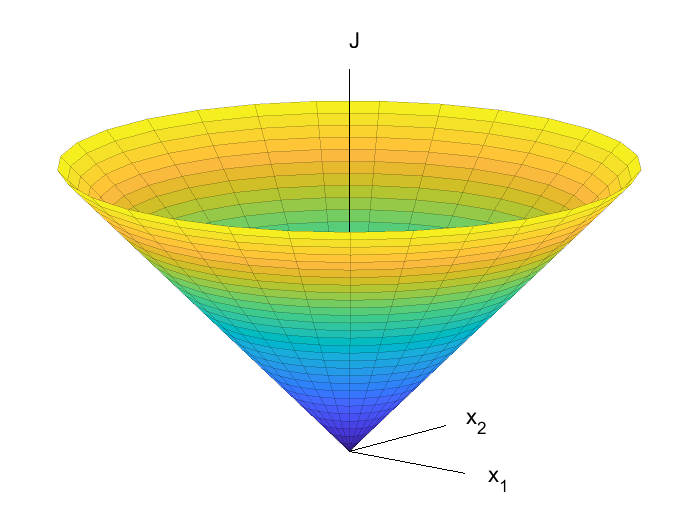
\includegraphics[width=0.7\linewidth]{norm}
%			\caption{}
			\label{fig:norm}
		\end{figure}
		
	\end{flushleft}
\end{frame}



\begin{frame}{Cone}
	% \framesubtitle{Parameter estimation}
	\begin{flushleft}
		
		The shape of the surface $\mathcal S = \{  (J, \bo{x}): \ J = || \bo{x} ||_2 \}$ is a \emph{cone}. We observe the following properties of a cone:
		
		\begin{itemize}
			\item There is a single tip point $\tau$ and a normal direction.
			
			\item  Slicing cone with planes orthogonal to the normal direction, we produce ellipsoids (we can call it tangent sets).
			
			\item For any point $p$ on the cone, the half-line from the tip point $\tau$ through $p$ lies on the cone.
		\end{itemize}
	
		\bigskip
	
		The tip point for $\mathcal S$ is $(0, \bo{0})$. Normal direction is $(n, \bo{0})$. Tangent sets are circles $|| \bo{x} ||_2 = h$, parameterized by $h$. 
		
		For any point $(J(\bo{p}), \bo{p})$ we can write half-line as $\mathcal L = \{ ( J(\gamma \bo{p}), \gamma \bo{p}): \ \gamma > 0 \}$.
		
		\begin{align}
			J(\gamma \bo{p}) = ||\gamma \bo{p}|| = \gamma ||\bo{p}|| = \gamma J(\bo{p})
		\end{align}
		
	\end{flushleft}
\end{frame}



\begin{frame}{Second-order cone}
	% \framesubtitle{Parameter estimation}
	\begin{flushleft}
		
		A second-order cone constraint has the following form:
		
		\begin{equation}
			||\bo{A}\bo{x}+\bo{b}|| \leq \bo{c}\T \bo{x} + d
		\end{equation}
		%
		where $\bo{A} \in \R^{n, n}$, $\bo{b}, \bo{c} \in \R^{n}$ and $d \in \R$.
		
		\bigskip
		
		This constraint describes interior of a cone. We can prove that surface of this set is is a cone described by the following equality:
		
		\begin{equation}
			||\bo{A}\bo{x}+\bo{b}|| = \bo{c}\T \bo{x} + d
		\end{equation}
	
	\end{flushleft}
\end{frame}



\begin{frame}{Second-order cone, linear 1}
	% \framesubtitle{Parameter estimation}
	\begin{flushleft}
		
		Let us consider the following simplified case:
		
		\begin{equation}
			\label{eq:Ac_cone}
			||\bo{A}\bo{x}|| = \bo{c}\T \bo{x}
		\end{equation}
		
		The tip of this cone is the point $\bo{x} = 0$, and the normal direction is $\bo{c}$.
		
		\bigskip
		
		Let us consider a point $\bo{p}$ that lies on the surface \eqref{eq:Ac_cone}: $||\bo{A}\bo{p}|| - \bo{c}\T \bo{p} = 0$. Clearly, a point $\gamma \bo{p}$ for $\gamma \geq 0$ lies on the same surface:
		
		\begin{align*}
			e = ||\bo{A}(\gamma\bo{p})|| - \bo{c}\T (\gamma \bo{p}) = 
			\gamma||\bo{A}\bo{p}|| - \gamma \bo{c}\T \bo{p} = \\
			= \gamma(||\bo{A}\bo{p}|| -\bo{c}\T \bo{p}) =0
		\end{align*}
		
		Therefore, the half-line going from tip $\bo{x} = 0$ through $\bo{p}$ lies on the cone. 
		
	\end{flushleft}
\end{frame}


\begin{frame}{Second-order cone, linear 2}
	% \framesubtitle{Parameter estimation}
	\begin{flushleft}
		
		We can consider plane $\mathcal P$ perpendicular to $\bo{c}$, distance $h / ||\bo{c}||$ away from the tip. All points on the plane are described as follows:
		
		\begin{align}
			\bo{x} = \frac{h}{||\bo{c}||^2} \bo{c} + \bo{T} \bo{z}, \ \ \forall \bo{z}
		\end{align}
		%
		where $\bo{T} = \text{null}(\bo{c}\T)$, so $\bo{c}\T\bo{T} = 0$. Then conic surface becomes:
		
		\begin{align}
			\left|\left|\bo{A}\frac{h}{||\bo{c}||^2} \bo{c} + \bo{A} \bo{T} \bo{z}\right|\right| = \bo{c}\T \left(\frac{h}{||\bo{c}||^2} \bo{c} + \bo{T} \bo{z} \right)
			\\ 
			||\bo{b}_0 + \bo{A} \bo{T} \bo{z}|| = h
		\end{align}
	%
	where $\bo{b}_0 = \frac{h}{||\bo{c}||^2} \bo{A} \bo{c}$. This is an ellipsoid. $\qed$
		
	\end{flushleft}
\end{frame}



\begin{frame}{Second-order cone, affine, 1}
	% \framesubtitle{Parameter estimation}
	\begin{flushleft}
		
		For a full second-order cone (SOC):
		%
		\begin{equation}
			||\bo{A}\bo{x}+\bo{b}|| = \bo{c}\T \bo{x} + d
		\end{equation}
	
		we can find a tip point; it corresponds to both right-hand side and left-hand side becoming zero:
		
		\begin{equation}
			\begin{cases}
				\bo{A}\bo{x}+\bo{b} = 0 \\
				\bo{c}\T \bo{x} + d = 0
			\end{cases}
		\end{equation}
		
		Given full rank matrix $\bo{A}$, the solution is $\bo{x} = -\bo{A}^{-1}\bo{b}$. The system would hold if:
		
		\begin{equation}
			-\bo{c}\T \bo{A}^{-1}\bo{b} + d = 0
		\end{equation}
		
		
	\end{flushleft}
\end{frame}



\begin{frame}{Second-order cone, affine, 2}
	% \framesubtitle{Parameter estimation}
	\begin{flushleft}
		
		Consider a point $\bo{p}_2$ on the surface $||\bo{A}\bo{p}_2+\bo{b}|| = \bo{c}\T \bo{p}_2 + d$. Let us consider an interval from tip $\bo{p}_1 = -\bo{A}^{-1}\bo{b}$ to $\bo{p}_2$:
		%
		\begin{equation}
			\bo{x} = \gamma \bo{p}_1 + (1 - \gamma) \bo{p}_2, \ \ \gamma \geq 0
		\end{equation}
		
		We can check if the points on the interval lie on the surface:
		%
		\begin{align*}
			e = ||\bo{A}\gamma \bo{p}_1+\bo{b} + \bo{A}(1 - \gamma) \bo{p}_2|| - (\gamma  \bo{c}\T\bo{p}_1 + d + (1 - \gamma)  \bo{c}\T\bo{p}_2)
		\end{align*}
	%
		\begin{align*}
			e = ||\gamma\bo{A} \bo{p}_1+\gamma\bo{b} + (1-\gamma)\bo{b} + \bo{A}(1 - \gamma) \bo{p}_2|| - \\ - (\gamma  \bo{c}\T\bo{p}_1 + \gamma d + (1-\gamma)d + (1 - \gamma)  \bo{c}\T\bo{p}_2)
		\end{align*}
		
		We know that $\bo{A}\gamma \bo{p}_1+\bo{b} = 0$ and $\bo{c}\T\bo{p}_1 + d = 0$:
		%
		\begin{align}
			e = || (1-\gamma)\bo{b} + \bo{A}(1 - \gamma) \bo{p}_2|| - (1-\gamma)d - (1 - \gamma)  \bo{c}\T\bo{p}_2
			\\
			e = || \bo{b} + \bo{A}\bo{p}_2|| - (d +\bo{c}\T\bo{p}_2) = 0
		\end{align}
		
		Thus, the interval (and therefore, the half-line on which it lies) lies on the surface.
		
	\end{flushleft}
\end{frame}



\begin{frame}{Second-order cone, affine, 3}
	% \framesubtitle{Parameter estimation}
	\begin{flushleft}
		
		Let us consider plane $\mathcal P$ perpendicular to $\bo{c}$, distance  $h / ||\bo{c}||$ away from the tip. All points on the plane are described as follows:
		
		\begin{align}
			\bo{x} = \frac{h}{||\bo{c}||^2} \bo{c} + \bo{T} \bo{z}, \ \ \forall \bo{z}
		\end{align}
		
		We can substitute it into the second-order cone:
		
		\begin{align}
			||\bo{A}(\frac{h}{||\bo{c}||^2} \bo{c} + \bo{T} \bo{z})+\bo{b}|| = \bo{c}\T (\frac{h}{||\bo{c}||^2} \bo{c} + \bo{T} \bo{z}) + d
			\\
			||\bo{b}_0+\bo{A}\bo{T} \bo{z}|| = h + d
		\end{align}
		%
			where $\bo{b}_0 = \frac{h}{||\bo{c}||^2} \bo{A} \bo{c}+\bo{b}$. This is an ellipsoid. $\qed$
	
		
	\end{flushleft}
\end{frame}




\begin{frame}{The role of the free constant, 1}
	% \framesubtitle{Parameter estimation}
	\begin{flushleft}
		
		Free constant $d$ plays a specific role in the SOC. As we said before, there is a condition $d = \bo{c}\T \bo{A}^{-1}\bo{b} + d$. We can explain it by looking at COS as intersection of two surfaces: 
		
		\begin{align}
			J = ||\bo{A}\bo{x}+\bo{b}|| \\
			P = \bo{c}\T \bo{x} + d
		\end{align}
		
		First is a cone and second is a plane. Their intersection is called a \emph{conic section}. 
				
	\end{flushleft}
\end{frame}




\begin{frame}{The role of the free constant, 2}
	% \framesubtitle{Parameter estimation}
	\begin{flushleft}
		
		Typical conic sections are shown below:
		
		% TODO: \usepackage{graphicx} required
		\begin{figure}
			\centering
			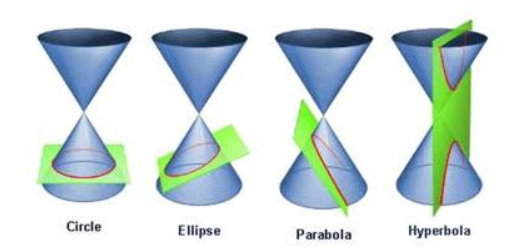
\includegraphics[width=0.7\linewidth]{cones}
			\label{fig:cones}
		\end{figure}
	
		As we can see, they represent ellipsoid and parabola. In order for them to represent a cone, the plane  $S$ needs to pass through the tip of the cone $J$. This can be achieved with the appropriate choice of constant $d$, which shifts $S$ up or down.
		
	\end{flushleft}
\end{frame}



\begin{frame}{Plotting level sets, 1}
	% \framesubtitle{Parameter estimation}
	\begin{flushleft}
		
		To plot a cone it is convenient to first use change of coordinates $\bo{y} = \bo{A}\bo{x}+\bo{b}$, meaning $\bo{x} =\bo{A}^{-1} (\bo{y} - \bo{b})$, giving us SOC:
		%
		\begin{equation}
			||\bo{y}|| = \bo{c}\T \bo{A}^{-1} (\bo{y} - \bo{b}) + d
		\end{equation}
		
		Note that $d - \bo{c}\T \bo{A}^{-1}\bo{b} = 0$ for a cone with a tip; so SOC becomes:
		%
		\begin{equation}
			||\bo{y}|| = \bo{c}\T \bo{A}^{-1} \bo{y}
		\end{equation}
		
		To plot level sets of this cone we choose height of the level set $h$ and pick point $\bo{y}_h = h \frac{\bo{A}^{-T} \bo{c}}{\bo{c}\T \bo{A}^{-1}\bo{A}^{-T} \bo{c}}$; we note that $\bo{c}\T \bo{A}^{-1} \bo{y}_h = h$. Then we consider points on the plane $\mathcal P$ orthogonal to $\bo{c}\T \bo{A}^{-1}$ and passing through $\bo{y}_h$:
		
		\begin{equation}
			\mathcal P = {\bo{y}_h + \bo{T}\bo{z}: \  \forall \bo{z}}
		\end{equation}
		 %
		 where $\bo{T} = \text{null}(\bo{c}\T \bo{A}^{-1})$, so $\bo{c}\T \bo{A}^{-1} \bo{T} = 0$.

	\end{flushleft}
\end{frame}


\begin{frame}{Plotting level sets, 2}
	% \framesubtitle{Parameter estimation}
	\begin{flushleft}
		
		Since  SOC becomes:
		%
		\begin{equation}
			||\bo{y}_h + \bo{T}\bo{z}|| = h
		\end{equation}
	
		Since $\bo{y}_h$ and $\bo{T}\bo{z}$ are orthogonal, it is equivalent to:
		%
		\begin{equation}
			||\bo{T}\bo{z}|| = g
		\end{equation}
	%
	where $g = \sqrt{ h^2 - \bo{y}_h\T\bo{y}_h }$. In the 3D case, this is a circle with radius $g$. We can find $N$ consecutive evenly spaced points of this circle, resulting in the next sequence of $\bo{y}_l$:
	
		\begin{align}
			\bo{y}_l &= \bo{y}_h + \bo{T}
			\begin{bmatrix}
				g\cos(\varphi) \\ -g\sin(\varphi)
			\end{bmatrix}, \ \ \ \varphi = 0, \ \frac{2\pi}{N},\ 2\frac{2\pi}{N}, \ ..., \ 2\pi 
		\\
		\bo{x}_l  &=\bo{A}^{-1} (\bo{y}_l - \bo{b})
		\end{align}
	
		The center of the ellipsoid representing this level set lies at the point $\bo{x} =\bo{A}^{-1} (\bo{y}_h - \bo{b})$.
		
	\end{flushleft}
\end{frame}



\begin{frame}{Plotting level sets, 3}
	% \framesubtitle{Parameter estimation}
	\begin{flushleft}
		
		
		\begin{figure}
			\centering
			\begin{subfigure}[b]{0.45\textwidth}
				\centering
				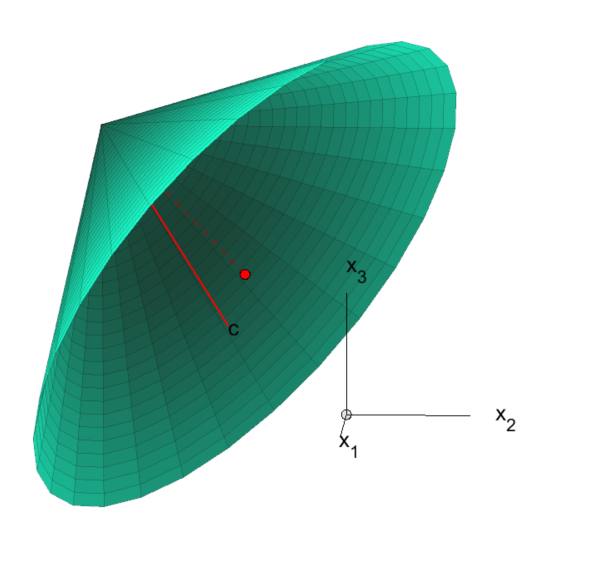
\includegraphics[width=\textwidth]{plotted1}
			\end{subfigure}
			\hfill
			\begin{subfigure}[b]{0.45\textwidth}
				\centering
				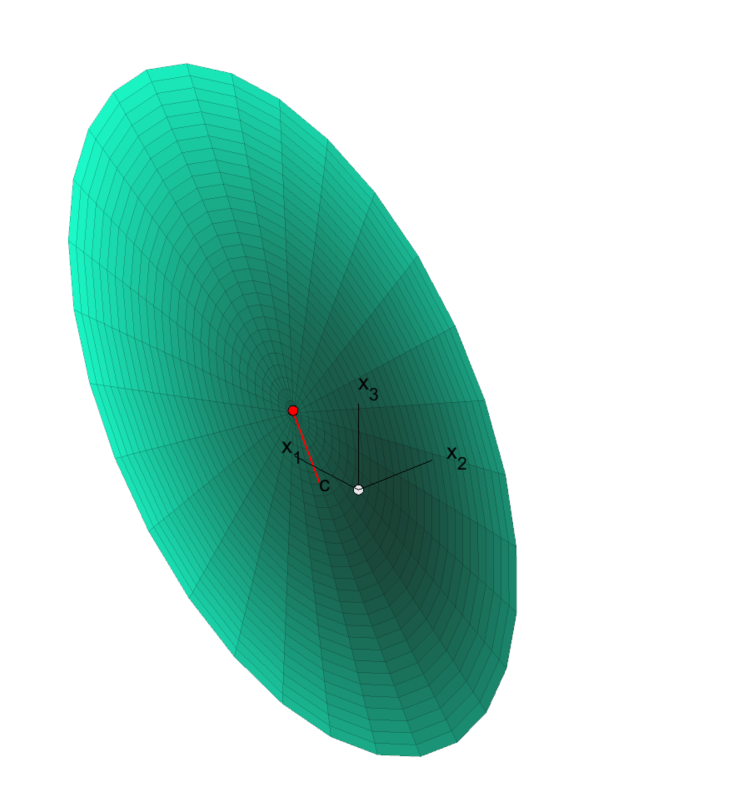
\includegraphics[width=\textwidth]{plotted2}
			\end{subfigure}
			\caption{Cone. Dashed line - centers of level-sets.}
		\end{figure}
		
	\end{flushleft}
\end{frame}




%\begin{frame}{Read more}
%	
%	\begin{itemize}
%		
%		\item ***
%		 
%		
%	\end{itemize}
%	
%\end{frame}



\myqrframe

\end{document}
